\chapter{Конструкторский раздел}
\label{cha:design}
В данном разделе будут рассмотрены схемы алгоритмов умножения матриц, введена модель вычисления трудоёмкости и в соответствии с ней подсчитана суммарная трудоёмкость для каждого из 3-х алгоритмов.\\
\textbf{Требования к вводу:}
\begin{itemize}
	\item на вход подаются 2 матрицы, и их размерности;
	\item передаётся результирующая матрица.
\end{itemize}
\textbf{Требования к программе:}
\begin{itemize}
	\item корректная обработка умножения матриц размерами 0 на 0;
	\item корректное умножение двух матриц.
\end{itemize}
\section{Схемы алгоритмов}
\label{sec:schemes}
На рисунках 2.1-2.3 представлены схемы алгоритмов умножения матриц.
\begin{figure}[H]
	\centering
	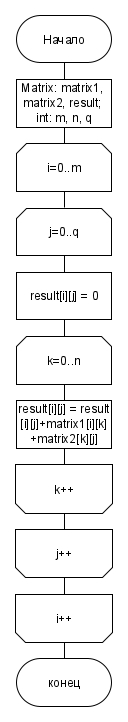
\includegraphics[height=0.7\textheight]{src/standard}
	\caption{Стандартный алгоритм}
	\label{fig:standard}
\end{figure}
\begin{figure}[H]
	\centering
	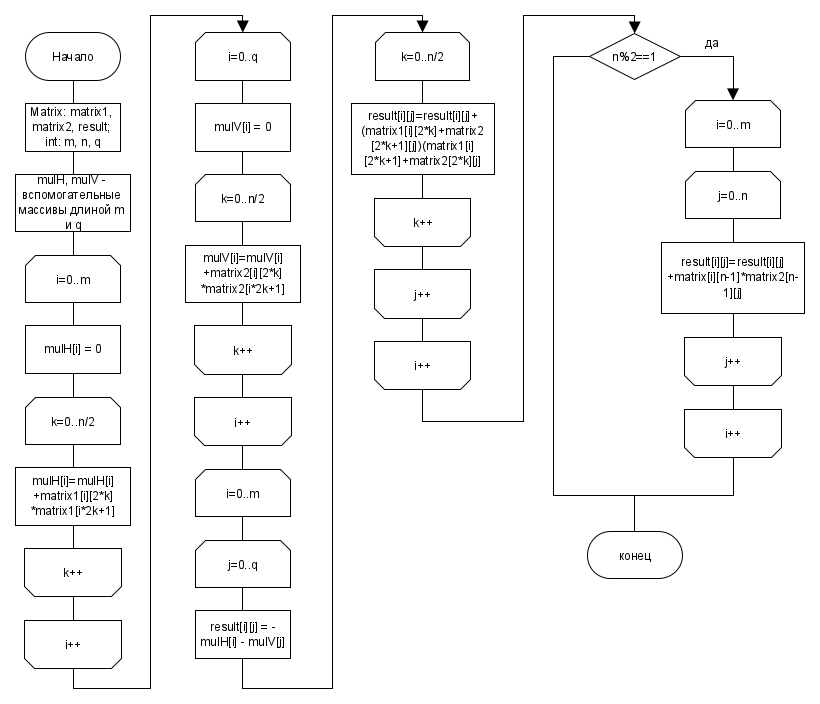
\includegraphics[width=1.05\linewidth]{src/winograd}
	\caption{Алгоритм Винограда}
	\label{fig:winograd}
\end{figure}
\begin{figure}[H]
	\centering
	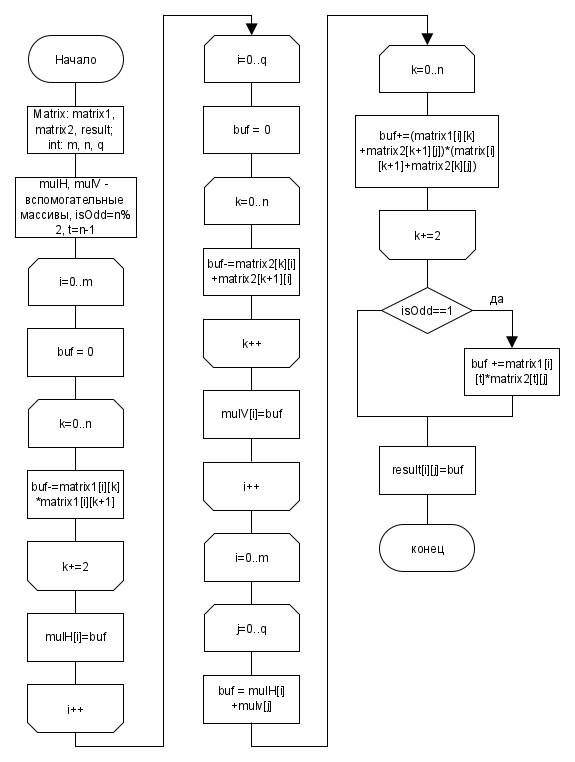
\includegraphics[width=1.05\linewidth]{src/winogradOptimized}
	\caption{Улучшенный алгоритм Винограда}
	\label{fig:winograd}
\end{figure}
\section{Трудоёмкость алгоритмов}
\label{sec:labour}
Введём модель вычислений трудоёмкости:
\begin{enumerate}[1)]
	\item стоимость базовых операций 1: =,+,-,*,==,!=,<,>,<=,>=>>\%,+=,-=,*=,/=,[],<<,>>;
	\item оценка трудоёмкости цикла $f_{for}=f_{init}+f_{comp}+N(f_{body}+f_{inc}+f_{comp})$;
	\item оценка трудоёмкости условного оператора, стоимость перехода положим 0, тогда
	\begin{equation}
f_{if}=f_{condition}+\begin{cases}
min(f_{1},f_{2})-\text{лучший случай}\\
max(f_{1},f_{2})-\text{худший случай}\\
\end{cases}
	\end{equation} 
\end{enumerate}
\paragraph{Классический алгоритм:}
\begin{equation}
f_{std}=2+M*(2+2+Q*(2+3+2+N*(2+8+1+1+1)))=13MNQ+7MQ+4M+2
\end{equation}
\paragraph{Алгоритм Винограда:}
\begin{enumerate}[I]
	\item Вычисление сумм произведений пар соседних элементов для каждой строки A:
	\begin{equation}
	f_{I}=2+M*(2+2+3+N/2*(3+1+6+2+3))=15/2MN+7M+2
	\end{equation}
	\item Вычисление сумм произведений пар соседних элементов для каждого столбца B аналогично:
	\begin{equation}
	f_{II}=15/2QN+7Q+2
	\end{equation}
	\item Заполнение $C_{ij}$:
	\begin{equation}
	f_{III}=2+M(2+2+Q(2+7+3+N/2(3+1+12+5+5)))=13MNQ+12MQ+4M+2
	\end{equation}
	\item Проверка нечётности N:
	\begin{equation}
	f_{IV}=2+\begin{cases}
	0-\text{лучший случай, N-чётное}\\
	13NQ+4M+2,-\text{худший случай, N-нечётное}
	\end{cases}
	\end{equation}
\end{enumerate}
Суммарная трудоёмкость:
\begin{equation}
\begin{split}
&f_{win}=f_{I}+f_{II}+f_{III}+f_{IV}=15/2MN+7M+2+15/2QN+7Q+2+\\
&+13MNQ+12MQ+4M+2+2+\begin{cases}0\\13NQ+4M+2\end{cases}=13MNQ+\\
&+12MQ+15/2MN+15/2QN+11M+7Q+8+\begin{cases}0\\13NQ+4M+2\end{cases}
\end{split}
\end{equation}
\paragraph{Улучшенный алгоритм винограда:}
\begin{enumerate}[I]
	\item Вычисление сумм произведений пар соседних элементов для каждой строки A:
	\begin{equation}
	f_{I}=2+M*(2+1+2+N/2*(2+4+2+1)+2)=9/2MN+7M+2
	\end{equation}
	\item Вычисление сумм произведений пар соседних элементов для каждого столбца B аналогично:
	\begin{equation}
	f_{II}=9/2QN+7Q+2
	\end{equation}
	\item Заполнение $C_{ij}$:
	\begin{equation}
	\begin{split}
	&f_{III}=2+M*(2+2+Q*(2+2+1+1+2+N/2*(2+8+4+1+1)+1+\\
	&+\begin{cases}0\\4+1+1\end{cases}+2+1))=8MNQ+MQ*(12+\begin{cases}0\\6\end{cases})+4M+2
	\end{split}
	\end{equation}
	\item Подсчёт констант: $f_{c}=1+1+1+1=4$
\end{enumerate}
Суммарная трудоёмкость:
\begin{equation}
\begin{split}
&f_{winopt}=9/2MN+7M+2+9/2QN+7Q+2+8MNQ+\\
&+MQ*(12+\begin{cases}0\\6\end{cases})+4M+2+4=\\
&=8MNQ+9/2MN+9/2QN+MQ*(12+\begin{cases}0\\6\end{cases})+11M+7Q+10
\end{split}
\end{equation}
\section{Вывод}
\label{sec:design_conclusion}
В данном разделе были рассмотрены схемы алгоритмов умножения матриц, введена модель вычисления трудоёмкости, рассчитаны трудоёмкости алгоритмов. Из формул 2.2, 2.7, 2.11 видно, что все три алгоритма зависят от размеров матриц как MNQ, однако, у оптимизированного алгоритма Винограда при этом слагаемом стоит наименьший коэффициент, равный 8, из чего следует, что он должен быть наиболее эффективным.
